\chapter{Implementación}

En un primer momento instalé en mi máquina Keras usando TensorFlow como backend, y ejecuté varios ejemplos en los que noté que dicha libreria es muy exigente si no se tiene una GPU y un procesador potente. Como no dispongo de una máquina con dichas características pensé en utilizar una AMI en Amazon EC2 especializada en `deep learning' con 2 GPU CUDA. 

\bigskip
Con dicha máquina los ejemplos se ejecutaban a muchísima velocidad y los tutoriales de la base de datos MNIST me daban resultados de 2,8\%. Dejé esa opción para más adelante por si pensaba competir con el resto de compañeros en cuando a rendimiento y me propuse utilizar algo que requiriera algo de programación por mi parte.

\bigskip
Probé DeepCL ya que mi máquina tiene una tarjeta Intel HD 5000 que soporta OpenCL, pero el rendimiento con los ejemplos no era demasiado bueno. Además según leí en varios artículos dicha librería tenía errores que hacía que no fuera todo lo óptima que debería ser.

\bigskip
Mas tarde probé la implementación en C ``minst-1lnn'' que resolvía el problema con una red neuronal muy simple y muy rápida. Pero los resultados no eran demasiado buenos ya que daba entorno al 5\% de error. Porté el código C a Python ya que es una buena forma de ver como funciona el algoritmo utilizado, pero aun dando los mismos resultados la ejecución del mismo era demasiado lenta como para ser usable.

\bigskip
También, tras leer algunos capítulos del libro ``Neural Networks and Deep Learning'' de Michael Nielsen, decidí probar algunos de los ejemplos ya que da el código base para una red neuronal multicapa bastante sencilla en Python y que se ejecutaba con bastante velocidad al utilizar la librería ``numpy''. 

\bigskip
Estuve utilizando como base los ejemplos de Michael Nielsen adaptándolos para la práctica y realizado diversas mejoras pero no conseguía bajar del resultado obtenido en la máquina AWS.

\bigskip
Así que tras muchas pruebas finalmente decidí volver a Keras en Amazon AWS probando muchas de las opciones que brinda la librería para conseguir un mejor resultado que el que dan los ejemplos proporcionados por la misma.

\bigskip
Los resultados obtenidos tras 12 épocas con los ejemplos de Keras era de un 99.25\% en el conjunto de prueba, con una tasa de error de 2.8\%. Para mejorar dichos resultados me propuse usar una configuración de capas más agresiva. En los ejemplos utilizaba una capa oculta de tipo convolucional con activación `relu' de 32 neuronas. Posteriormente fui agregando capas convolucionales duplicando las neuronas de cada una de ellas. Este tipo de configuración requería mas tiempo de proceso pero al final la red sobreaprendía demasiado y aunque daba un error del 0.0\% en el conjunto de entrenamiento daba unos resultados parecidos a los de los ejemplos en el conjunto de prueba.

\bigskip
La estructura de datos utilizada por Keras está organizada por capas, permitiendo de forma fácil ir agregando capas de diferentes tipos. Además tiene una cantidad enorme de tipos de capas predefinidos. Tenemos capas de activación, capas softmax, capas lineales y muchísimos tipos mas que podemos ir agregando de forma sencilla.
 
\bigskip
La primera capa que agreguemos será la que se defina como capa de entrada y deberá tener el mismo tamaño que los datos de entrada. La segunda capa toma la salida de la primera y establece las dimensiones de salida. Esto significa que la segunda capa tiene tantos nodos como tiene su salida. Esta configuración se irá encadenando hasta la capa de salida que en nuestro caso es de 10 (los números del 0 al 9 que vamos a reconocer).

\bigskip
Una vez que tengamos nuestro modelo debemos compilarlo. La compilación utiliza las librerías del backend utilizado (en nuestro caso TensorFlow). El backend selecciona automáticamente la mejor forma de representar la red para el entrenamiento, y hará que las predicciones se ejecuten en el hardware disponible de la forma mas óptima utilizando la GPU si está disponible.

\bigskip
Al la hora de compilar debemos indicar algunas propiedades adicionales para entrenar la red, como la función de pérdida (loss) el número de épocas así como optimizador utilizado para buscar en diferentes pesos de la red o cualquier métrica opcional que deseemos recopilar durante el entrenamiento. En nuestras pruebas hemos probado diferentes funciones loss así como optimizadores. Para esta práctica como los datos están categorizados hemos utilizado la función categorical\_crossentropy pues es la mas adecuada en base a nuestros datos pues  están categorizados. De igual forma podemos elegir el algoritmo optimizador, hemos probado `sgd' (stocastic gradient descent), `adam' y `adadelta' siendo este último el que nos ha dado mejores resultados. 


\bigskip
La fase de entrenamiento se ejecutará en un número fijo de iteraciones a través del conjunto de datos llamado `epochs' (épocas). Definiremos tamaño del lote o numero de imágenes que se evaluarán antes de que se realice una actualización de pesos en la red con el argumento batch\_size. 

\bigskip
Una vez entrenada nuestra red neuronal ya podemos evaluar su eficiencia utilizando el conjunto de datos de prueba.

\section{Configuracion final}

Tras varias pruebas, mi implementación final fue la siguiente:
\begin{itemize}
	\item \textbf{Número de capas}: Ocho capas.
	\item \textbf{Tamaño de capa de entrada}: 28x28. Tantas neuronas como píxeles en la imagen
	\item \textbf{Tamaño de capa de salida}: 10. Tantas neuronas como posibles soluciones. 
	\item \textbf{Función de activación}: relu
	\item \textbf{Tipo de aprendizaje}: Estocástico. Reajuste de pesos tras cada imagen
\end{itemize}


\section{Definición de capas} 

\begin{itemize}
	\item La primera capa oculta es una capa convolucional llamada Convolution2D. La capa tiene 32 mapas característicos, que con el tamaño de 5×5 y una función de activación del rectificador. Esta es la capa de entrada.
	\item A continuación definimos una capa de 'pooling' que toma el máximo llamado MaxPooling2D. Está configurado con un tamaño de pool de 2×2.
	\item Capa convolucional con 15 mapas de características de tamaño 3×3.
	\item La siguiente capa es una capa de regularización que utiliza una deserción llamada "Dropout". Está configurado para excluir aleatoriamente el 20\% de las neuronas en la capa para reducir el exceso de sobreaprendizaje.
	\item A continuación se convierte la capa que convierte los datos de la matriz 2D en un vector llamado "Flatten". Permite que la salida sea procesada por capas estándar completamente conectadas.
	\item A continuación, una capa completamente conectada con 128 neuronas y función de activación del rectificador.
	\item Capa totalmente conectada con 50 neuronas y activación del rectificador.
	\item Por último, la capa de salida tiene 10 neuronas para las 10 clases y una función de activación softmax para emitir predicciones probabilisticas para cada clase.
\end{itemize}


En la figura \ref{fig:model} podemos ver como están definidas las capas.

\begin{figure}[H]
\centering
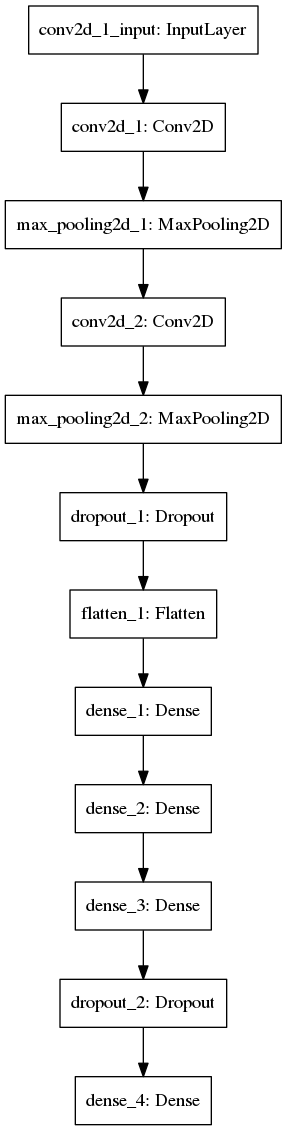
\includegraphics[width=0.5\textwidth]{../images/model}
\caption{Diagrama con las capas utilizadas}
\label{fig:model}
\end{figure}








